%% =============================================================================
%% RESULTS SECTION - Adaptive Caliper Selection in Propensity Score Matching
%% =============================================================================

\section{Results}

We evaluated the proposed adaptive caliper selection (ACS) framework through Monte Carlo simulation ($R=100$ replications) under a scenario with $n=1000$ observations, 50\% treatment prevalence, medium overlap, and strong confounding. The true treatment effect was $\tau=0.5$.

%% -----------------------------------------------------------------------------
\subsection{Propensity Score Estimation and Overlap}

Figure~\ref{fig:ps_distribution} displays the estimated propensity score distributions by treatment group. Substantial overlap exists between treated and control units, though separation is evident---consistent with the moderate overlap specification. The correlation between true and estimated propensity scores was $\rho = 0.98$, indicating accurate PS estimation.

\begin{figure}[htbp]
    \centering
    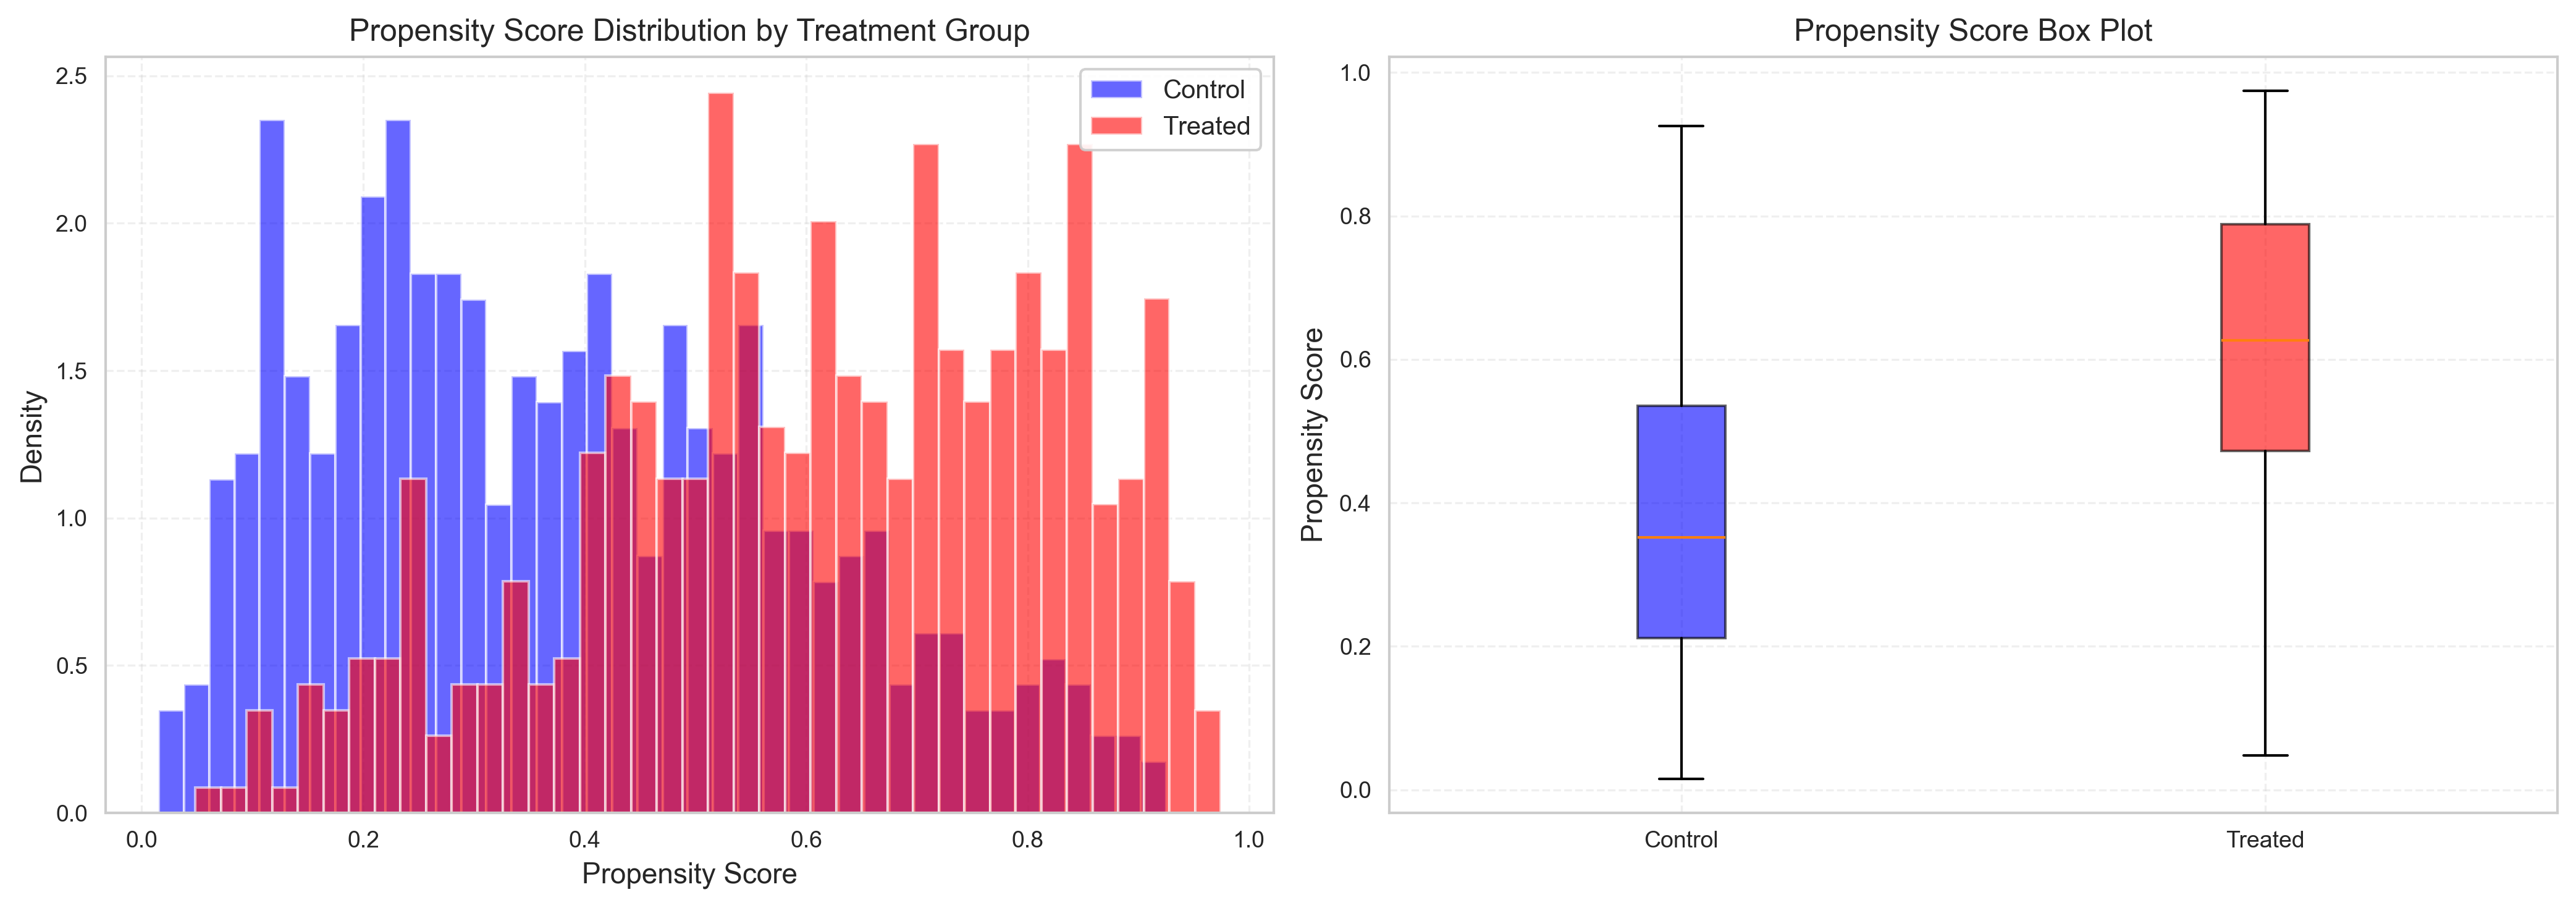
\includegraphics[width=0.95\textwidth]{outputs/figures/fig1_ps_distribution.png}
    \caption{Propensity score distribution by treatment group. Left: overlapping histograms showing density. Right: box plots illustrating median, interquartile range, and outliers.}
    \label{fig:ps_distribution}
\end{figure}

%% -----------------------------------------------------------------------------
\subsection{Pareto Frontier Characterization}

The multi-objective trade-off between covariate balance $B(c)$ and sample retention $R(c)$ is visualized in Figure~\ref{fig:pareto_frontier}. We evaluated 20 caliper values ranging from $c=0.05$ to $c=2.0$ standard deviations. Table~\ref{tab:pareto_frontier} presents the Pareto-optimal caliper values.

\begin{figure}[htbp]
    \centering
    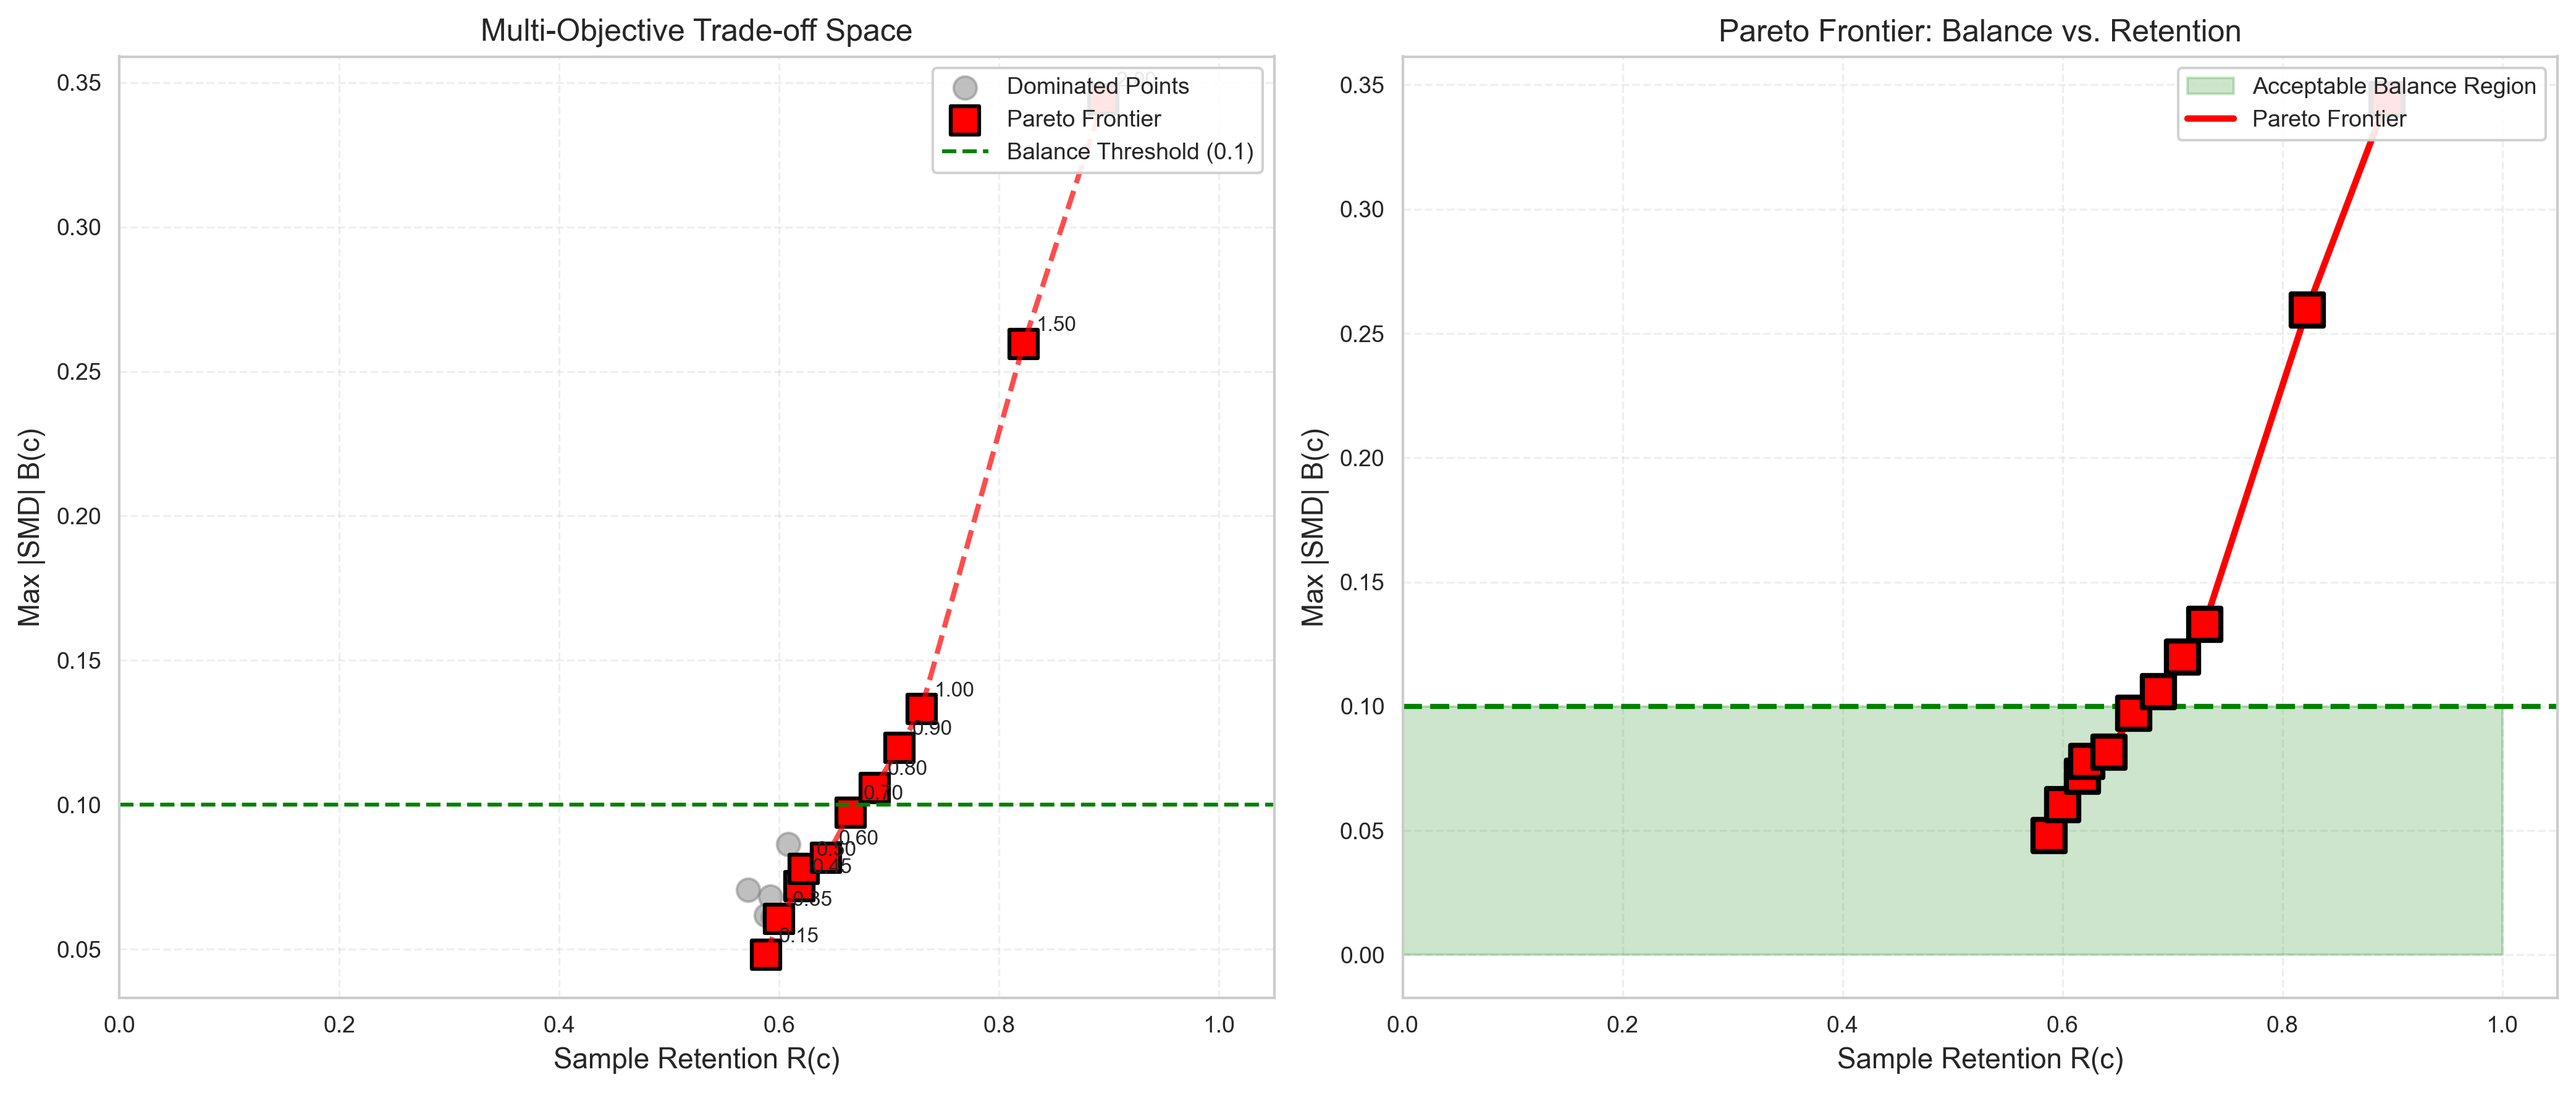
\includegraphics[width=0.95\textwidth]{outputs/figures/fig2_pareto_frontier.png}
    \caption{Multi-objective trade-off space. Left: all evaluated calipers with Pareto frontier highlighted. Right: Pareto frontier with acceptable balance region (max $|\text{SMD}| \leq 0.1$) shaded.}
    \label{fig:pareto_frontier}
\end{figure}

\begin{table}[htbp]
    \centering
    \caption{Pareto frontier: optimal trade-off points between balance and retention.}
    \label{tab:pareto_frontier}
    \begin{tabular}{cccc}
        \toprule
        Caliper (SD) & Max $|\text{SMD}|$ & Retention & $n$ Matched \\
        \midrule
        0.15 & 0.048 & 0.588 & 291 \\
        0.35 & 0.061 & 0.600 & 297 \\
        0.45 & 0.072 & 0.618 & 306 \\
        0.50 & 0.078 & 0.622 & 308 \\
        0.60 & 0.082 & 0.642 & 318 \\
        0.70 & 0.097 & 0.665 & 329 \\
        0.80 & 0.106 & 0.687 & 340 \\
        0.90 & 0.120 & 0.709 & 351 \\
        1.00 & 0.133 & 0.729 & 361 \\
        1.50 & 0.259 & 0.822 & 407 \\
        2.00 & 0.344 & 0.895 & 443 \\
        \bottomrule
    \end{tabular}
\end{table}

The frontier exhibits the expected monotonic trade-off: smaller calipers achieve better balance (lower max $|\text{SMD}|$) at the cost of reduced retention. Notably, calipers below $c=0.70$ SD achieve the conventional balance threshold of $|\text{SMD}| \leq 0.10$.

%% -----------------------------------------------------------------------------
\subsection{Optimal Caliper Selection by Criterion}

Table~\ref{tab:optimal_calipers} compares the three ACS selection criteria. Figure~\ref{fig:optimal_selection} visualizes these selections on the Pareto frontier.

\begin{table}[htbp]
    \centering
    \caption{Optimal caliper selection by criterion ($\tau_{\text{balance}} = 0.10$, $\lambda = 0.5$).}
    \label{tab:optimal_calipers}
    \begin{tabular}{lccccl}
        \toprule
        Criterion & Caliper (SD) & Max $|\text{SMD}|$ & Retention & $n$ Matched & Threshold Met \\
        \midrule
        ACS-Balance  & 0.70 & 0.097 & 66.5\% & 329 & Yes \\
        ACS-Knee     & 0.50 & 0.078 & 62.2\% & 308 & Yes \\
        ACS-Weighted & 1.00 & 0.133 & 72.9\% & 361 & No \\
        \bottomrule
    \end{tabular}
\end{table}

\begin{figure}[htbp]
    \centering
    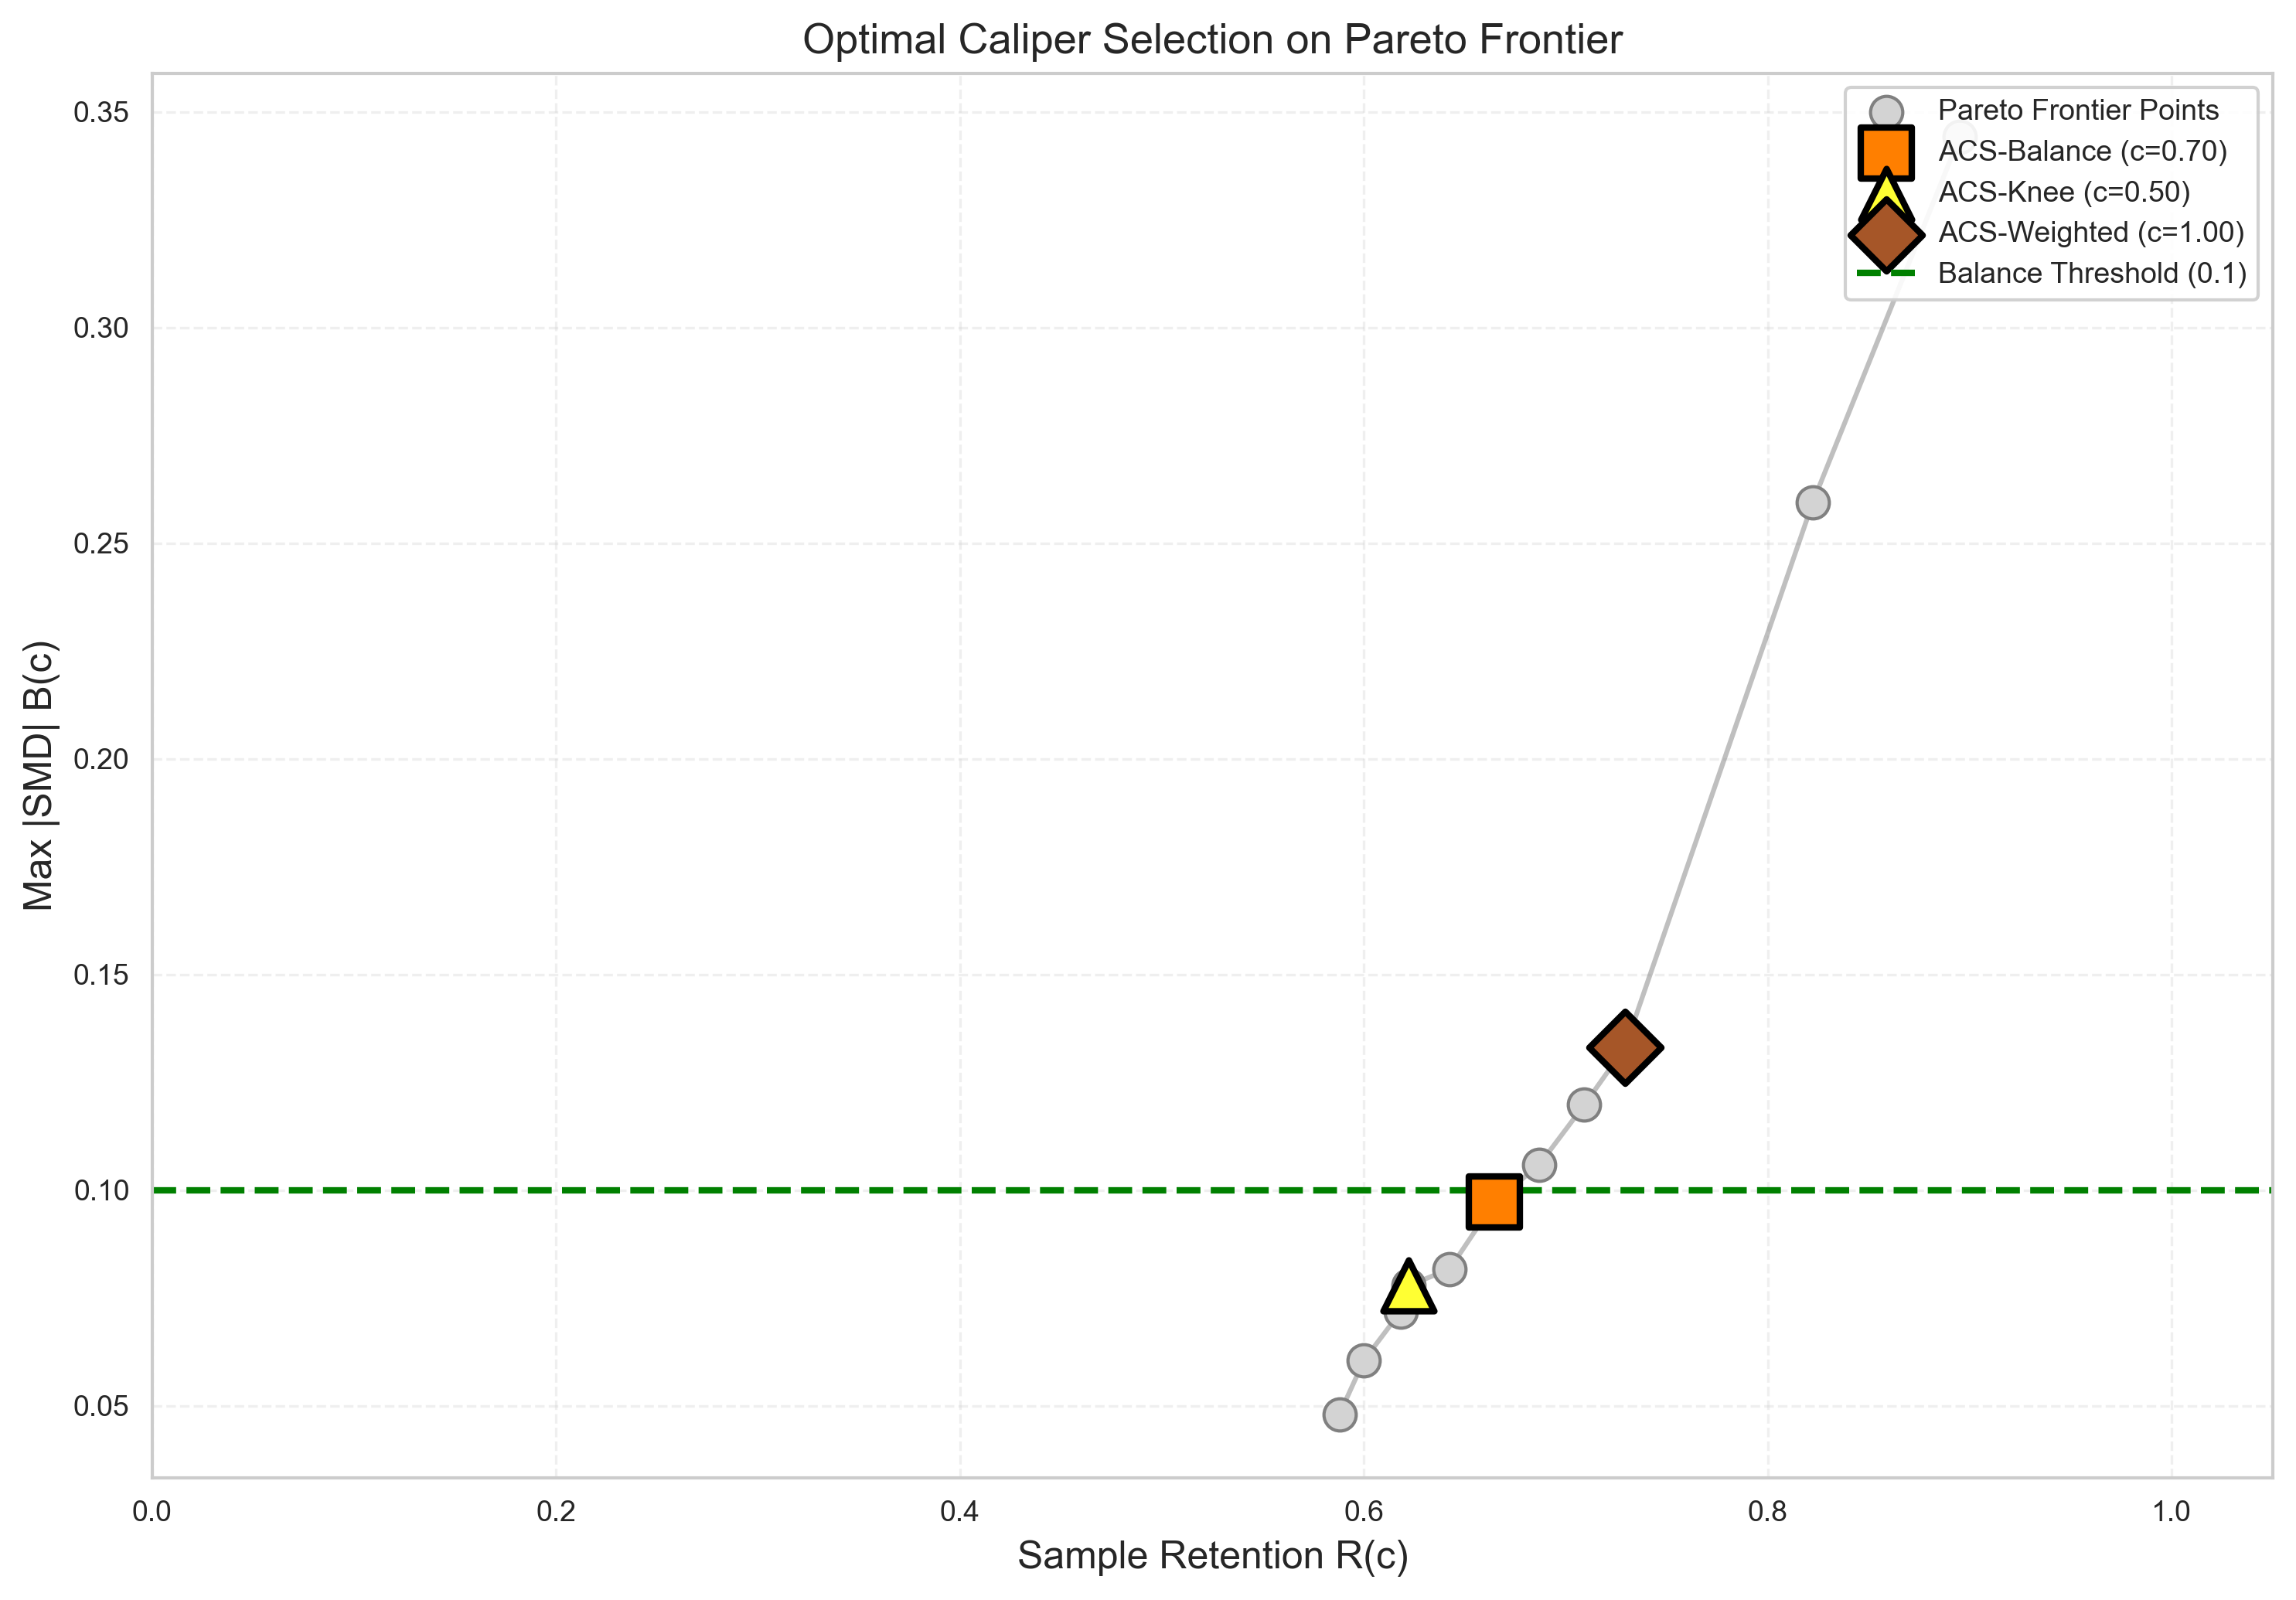
\includegraphics[width=0.75\textwidth]{outputs/figures/fig3_optimal_caliper_selection.png}
    \caption{Optimal caliper selections on the Pareto frontier. ACS-Balance selects the largest caliper meeting the balance threshold; ACS-Knee identifies the point of maximum curvature; ACS-Weighted minimizes a weighted objective.}
    \label{fig:optimal_selection}
\end{figure}

The ACS-Balance criterion selected $c^* = 0.70$ SD---the largest caliper achieving $|\text{SMD}| \leq 0.10$---yielding 329 matched pairs (66.5\% retention). ACS-Knee selected a more conservative $c^* = 0.50$ SD, sacrificing 21 pairs for improved balance (max $|\text{SMD}| = 0.078$). ACS-Weighted, prioritizing retention equally with balance, selected $c^* = 1.00$ SD but failed to meet the balance threshold.

%% -----------------------------------------------------------------------------
\subsection{Covariate Balance Improvement}

Table~\ref{tab:balance_comparison} presents standardized mean differences before and after matching using the ACS-Balance caliper ($c = 0.70$ SD). Figure~\ref{fig:love_plot} visualizes these improvements.

\begin{table}[htbp]
    \centering
    \caption{Covariate balance before and after matching (ACS-Balance, $c = 0.70$ SD).}
    \label{tab:balance_comparison}
    \begin{tabular}{lcccc}
        \toprule
        Covariate & $|\text{SMD}|$ Before & $|\text{SMD}|$ After & Improvement (\%) \\
        \midrule
        $X_1$ & 0.508 & 0.089 & 82.5 \\
        $X_2$ & 0.457 & 0.053 & 88.4 \\
        $X_3$ & 0.450 & 0.028 & 93.8 \\
        $X_4$ & 0.340 & 0.073 & 78.6 \\
        $X_5$ & 0.176 & 0.097 & 44.7 \\
        $X_6$ & 0.365 & 0.061 & 83.4 \\
        \midrule
        \textbf{Max} & \textbf{0.508} & \textbf{0.097} & \textbf{80.9} \\
        \bottomrule
    \end{tabular}
\end{table}

\begin{figure}[htbp]
    \centering
    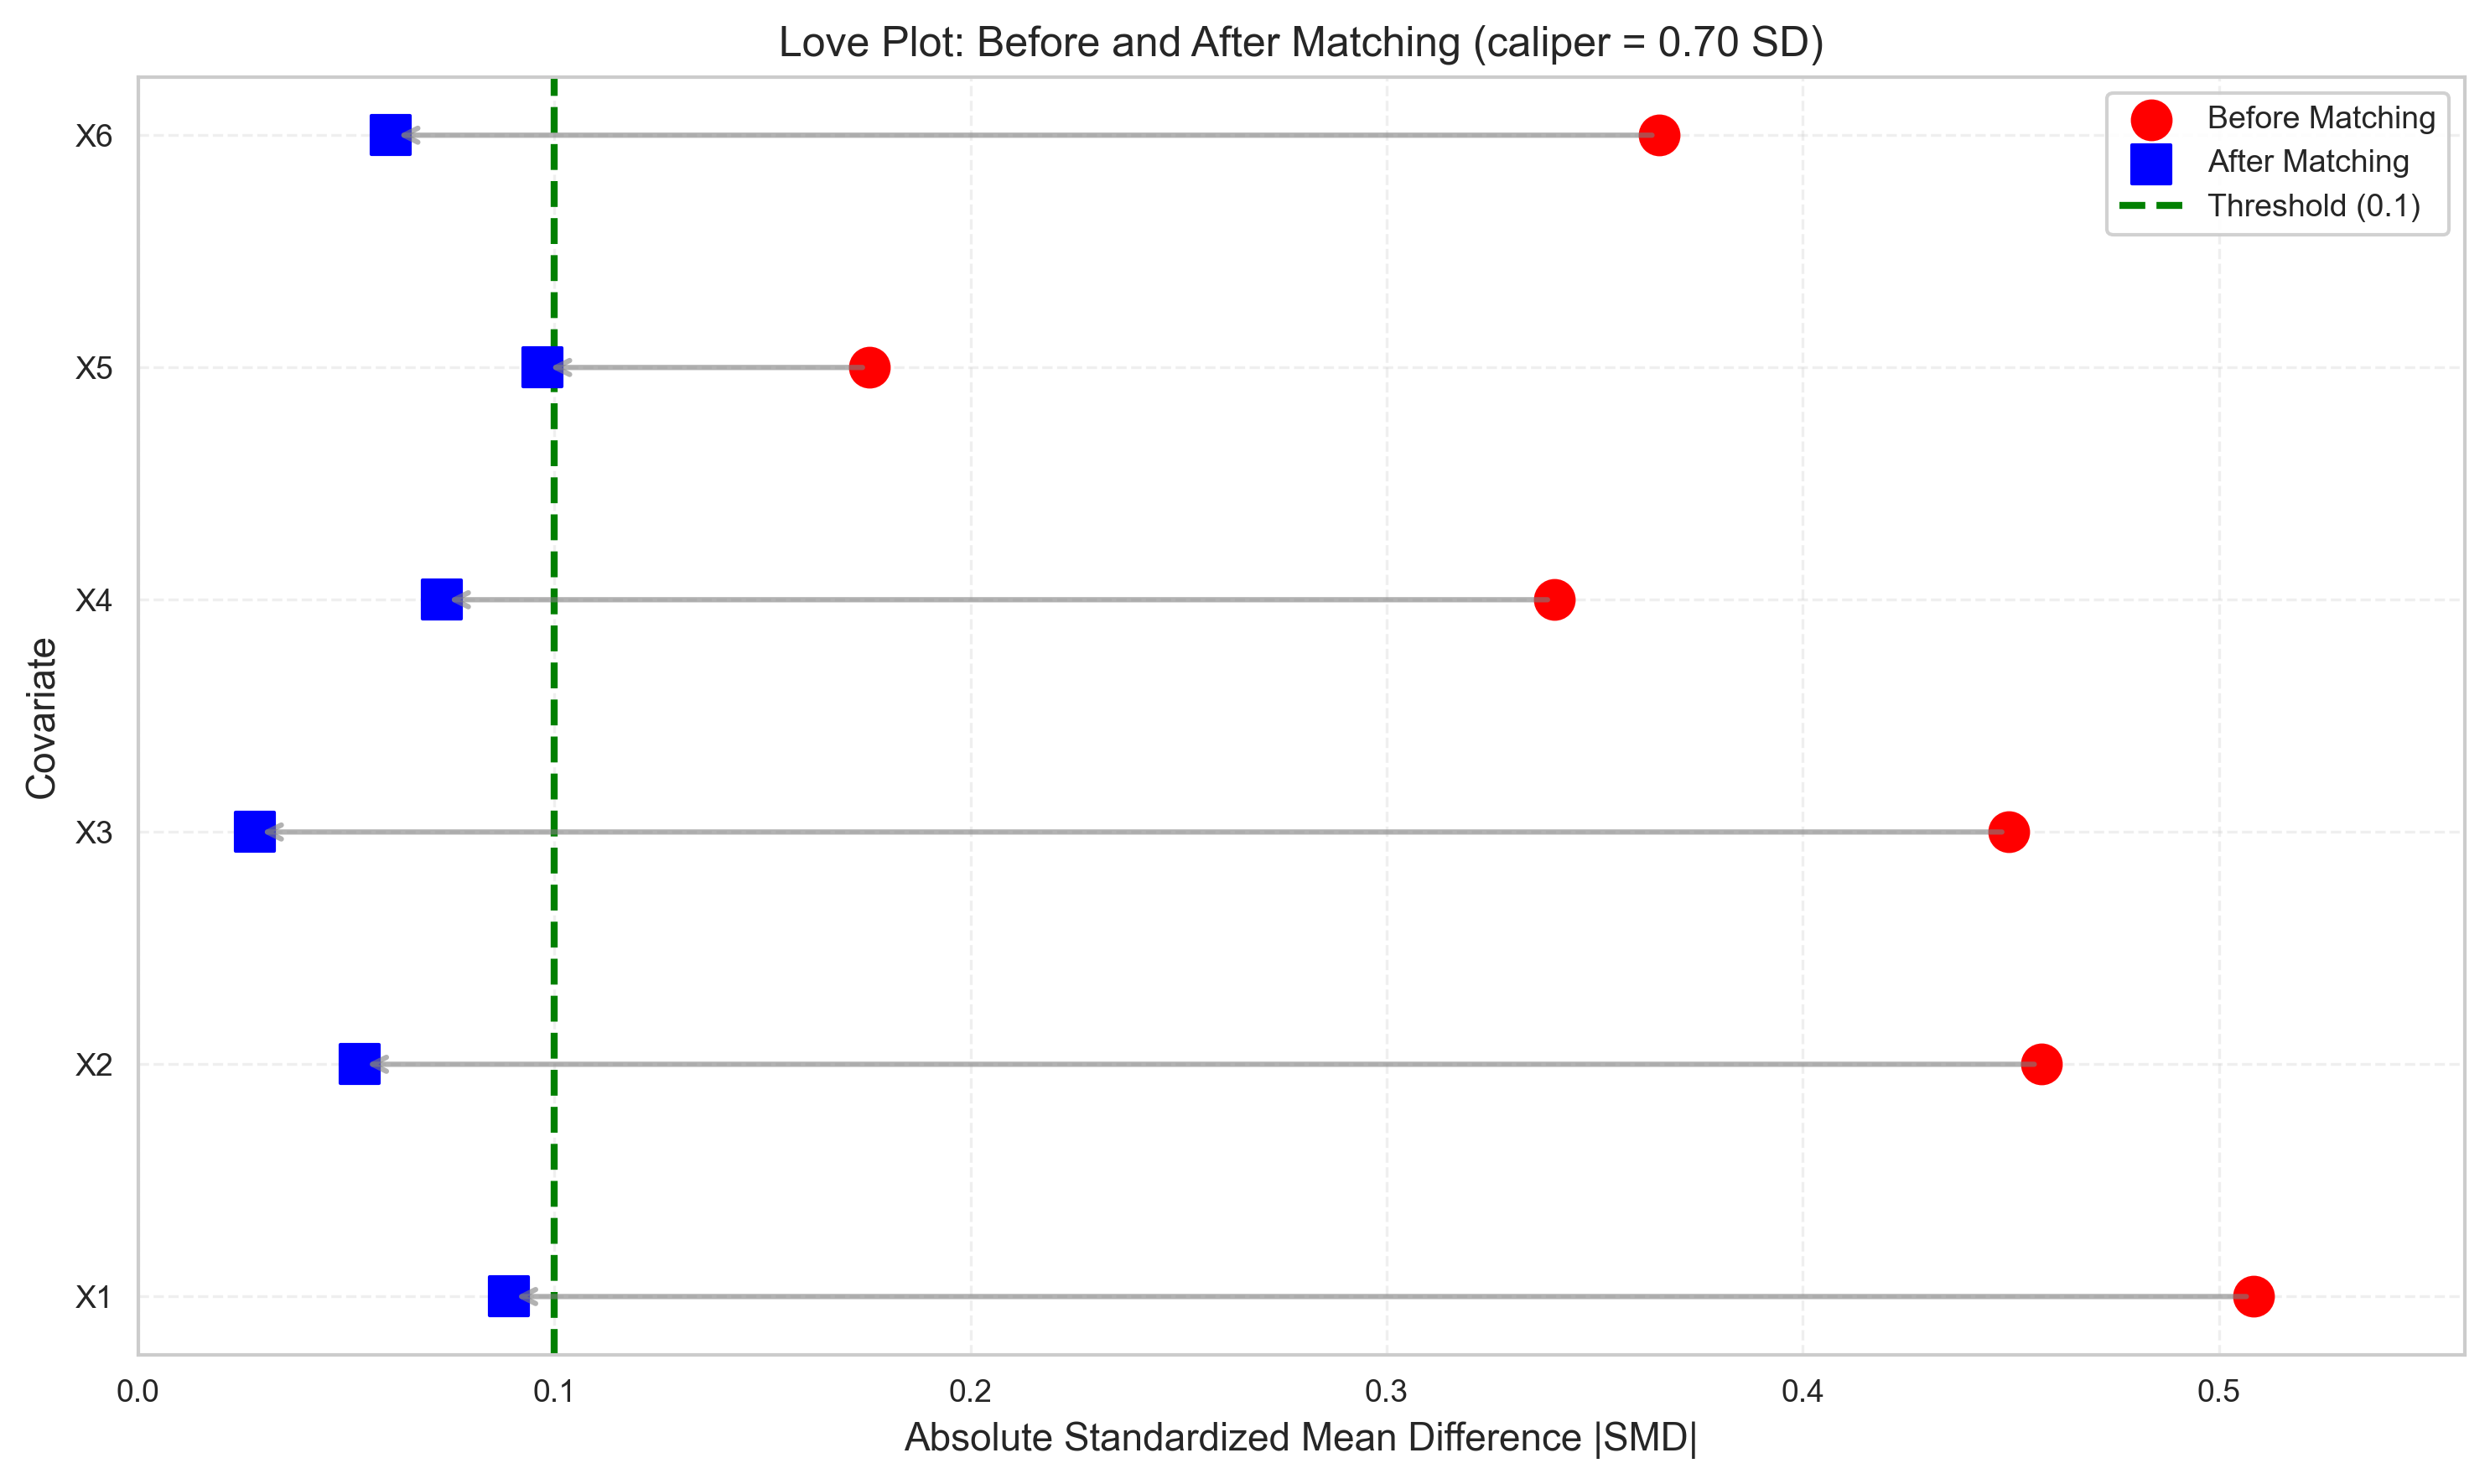
\includegraphics[width=0.75\textwidth]{outputs/figures/fig4_love_plot.png}
    \caption{Love plot showing covariate balance before (circles) and after (squares) matching. Arrows indicate direction and magnitude of improvement. Dashed line: balance threshold ($|\text{SMD}| = 0.10$).}
    \label{fig:love_plot}
\end{figure}

Matching substantially reduced imbalance across all covariates. The maximum $|\text{SMD}|$ decreased from 0.508 to 0.097---an 81\% reduction. All covariates achieved balance below the 0.10 threshold, with improvements ranging from 45\% ($X_5$) to 94\% ($X_3$).

%% -----------------------------------------------------------------------------
\subsection{Treatment Effect Estimation}

Table~\ref{tab:treatment_effects} compares ATT estimates across methods. Figure~\ref{fig:te_estimates} displays point estimates with 95\% confidence intervals.

\begin{table}[htbp]
    \centering
    \caption{Treatment effect estimation comparison (true ATT $= 0.50$).}
    \label{tab:treatment_effects}
    \begin{tabular}{lccccc}
        \toprule
        Method & Caliper & $n$ Matched & $\widehat{\text{ATT}}$ & Bias & 95\% CI \\
        \midrule
        ACS-Balance  & 0.70 & 329 & 0.607 & 0.107 & [0.389, 0.825] \\
        ACS-Knee     & 0.50 & 308 & 0.521 & 0.021 & [0.309, 0.733] \\
        ACS-Weighted & 1.00 & 361 & 0.758 & 0.258 & [0.553, 0.963] \\
        Fixed-0.1    & 0.10 & 291 & 0.414 & $-$0.086 & [0.192, 0.636] \\
        Fixed-0.2    & 0.20 & 291 & 0.432 & $-$0.068 & [0.205, 0.660] \\
        Fixed-0.5    & 0.50 & 308 & 0.521 & 0.021 & [0.309, 0.733] \\
        \bottomrule
    \end{tabular}
\end{table}

\begin{figure}[htbp]
    \centering
    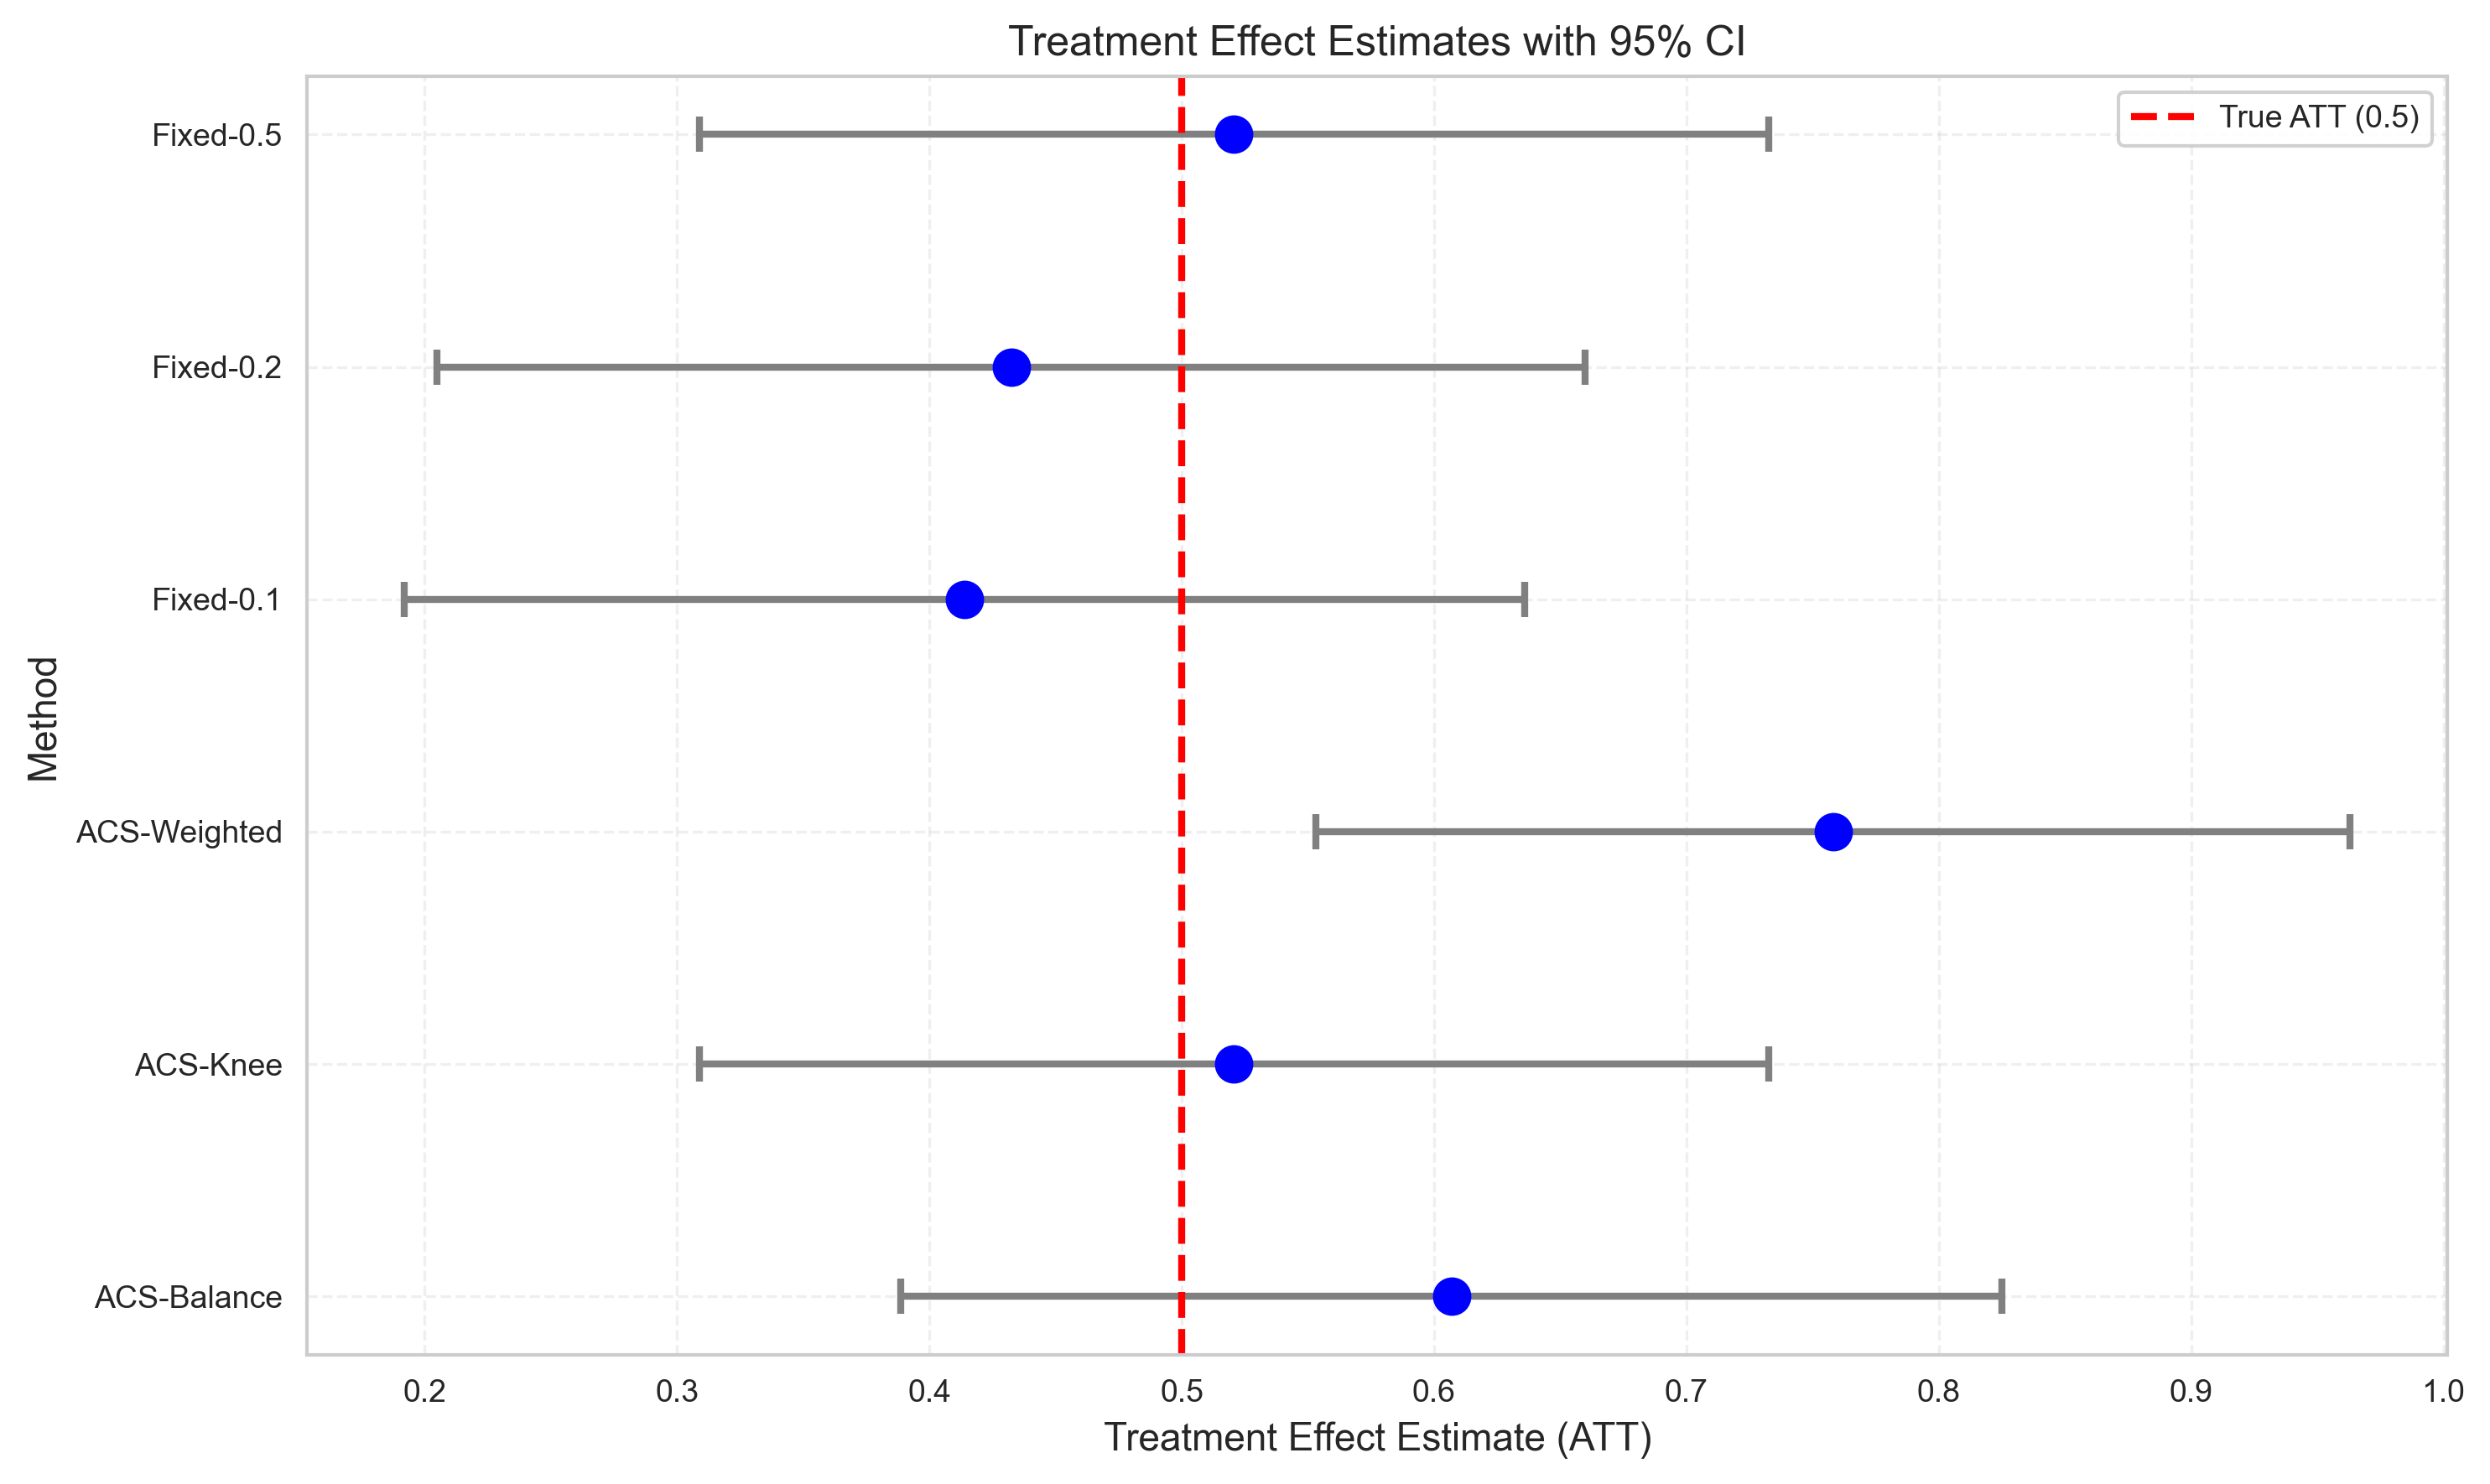
\includegraphics[width=0.75\textwidth]{outputs/figures/fig5_treatment_effect_estimates.png}
    \caption{Treatment effect estimates with 95\% confidence intervals. Dashed line indicates true ATT ($\tau = 0.50$).}
    \label{fig:te_estimates}
\end{figure}

ACS-Knee achieved the smallest bias (0.021), closely followed by Fixed-0.5 (identical selection in this realization). ACS-Balance exhibited moderate bias (0.107), while ACS-Weighted showed substantial bias (0.258) due to inadequate balance. Fixed calipers (0.1, 0.2) produced negative bias, likely due to over-restriction. All confidence intervals except ACS-Weighted covered the true effect.

%% -----------------------------------------------------------------------------
\subsection{Monte Carlo Simulation Results}

Table~\ref{tab:monte_carlo} summarizes performance across 100 replications. Figure~\ref{fig:mc_results} displays the distributions of key metrics.

\begin{table}[htbp]
    \centering
    \caption{Monte Carlo simulation results ($R = 100$ replications, true ATT $= 0.50$).}
    \label{tab:monte_carlo}
    \resizebox{\textwidth}{!}{%
    \begin{tabular}{lcccccccc}
        \toprule
        Method & $\bar{n}$ (SD) & Retention & Max $|\text{SMD}|$ & Mean Bias & $|\text{Bias}|$ & RMSE & MSE & Coverage \\
        \midrule
        Fixed-0.1    & 300 (14) & 61.4\% & 0.063 & $-$0.002 & 0.070 & 0.089 & 0.019 & 99\% \\
        Fixed-0.2    & 304 (13) & 62.2\% & 0.062 & 0.011 & 0.068 & 0.089 & 0.019 & 98\% \\
        Fixed-0.5    & 321 (12) & 65.8\% & 0.078 & 0.096 & 0.112 & 0.130 & 0.027 & 89\% \\
        No Caliper   & 489 (9)  & 100\%  & 0.518 & 1.341 & 1.341 & 1.354 & 1.832 & 0\% \\
        \midrule
        ACS-Balance  & 332 (20) & 68.0\% & 0.090 & 0.154 & 0.161 & 0.184 & 0.044 & 65\% \\
        ACS-Knee     & 325 (19) & 66.6\% & 0.080 & 0.116 & 0.133 & 0.170 & 0.039 & 74\% \\
        ACS-Weighted & 362 (27) & 74.2\% & 0.141 & 0.327 & 0.329 & 0.376 & 0.151 & 23\% \\
        \bottomrule
    \end{tabular}%
    }
\end{table}

\begin{figure}[htbp]
    \centering
    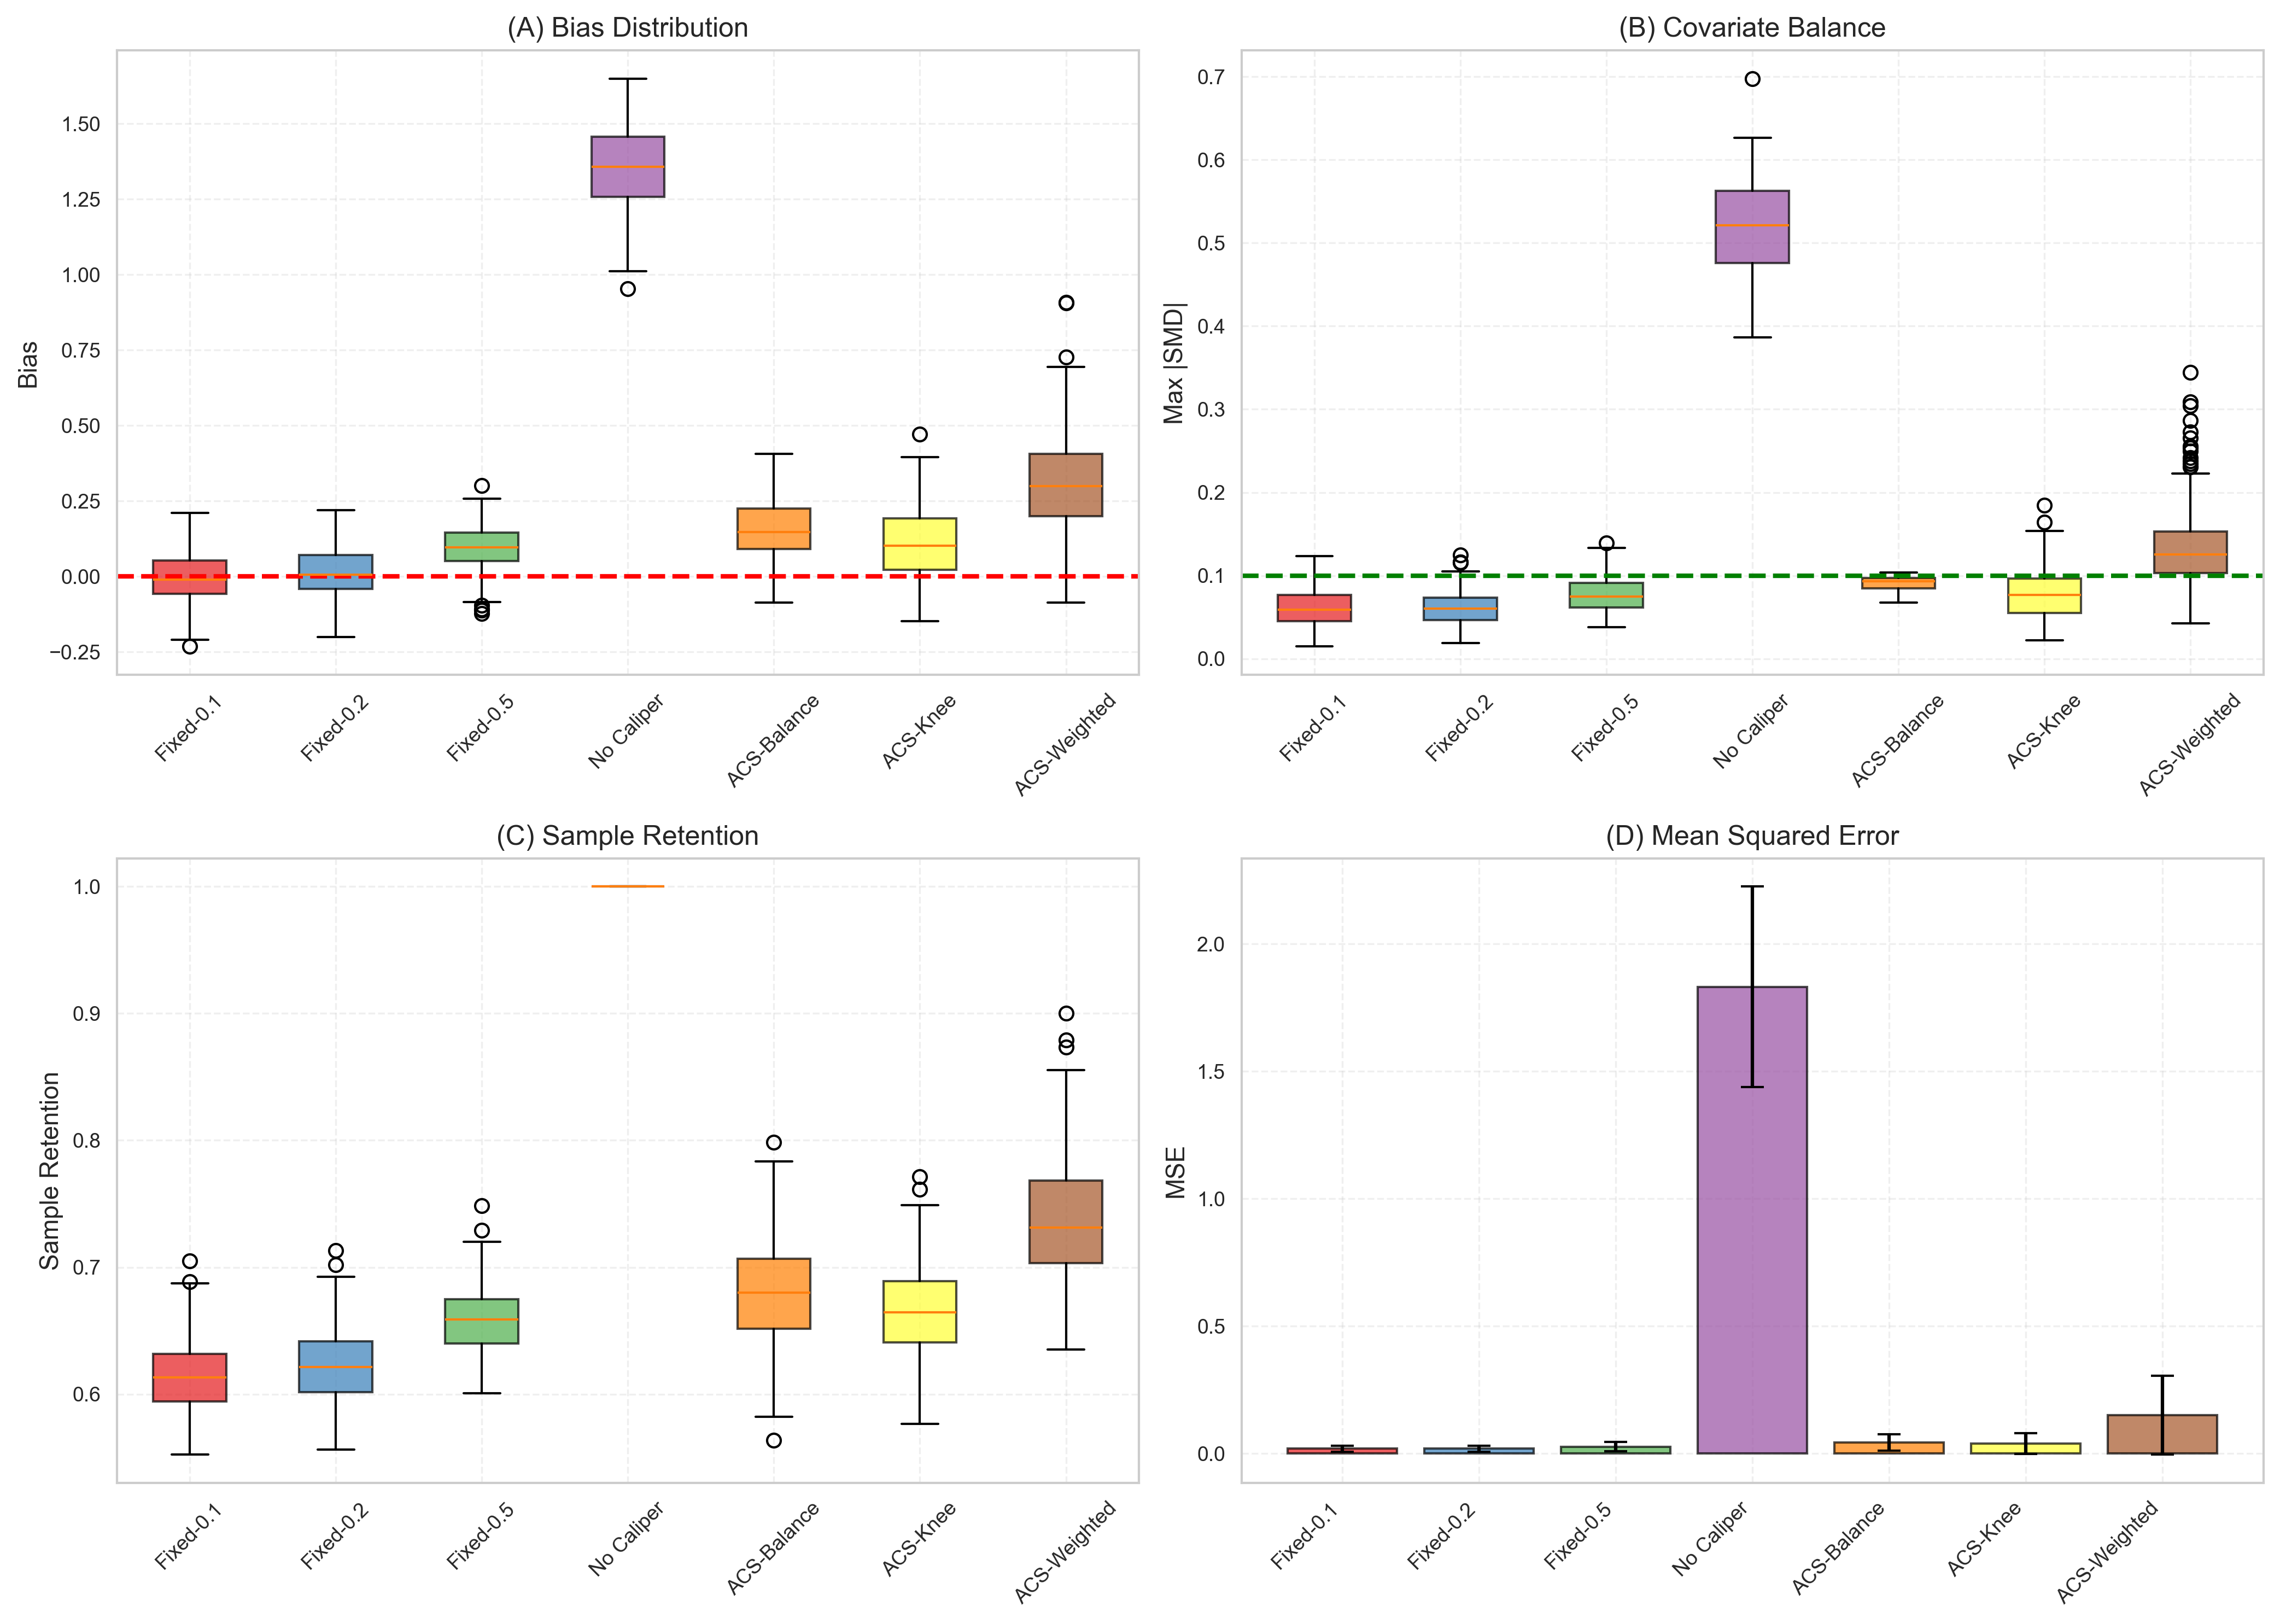
\includegraphics[width=0.95\textwidth]{outputs/figures/fig6_monte_carlo_results.png}
    \caption{Monte Carlo results. (A) Bias distribution by method. (B) Covariate balance (max $|\text{SMD}|$). (C) Sample retention. (D) Mean squared error.}
    \label{fig:mc_results}
\end{figure}

\subsubsection{Balance-Bias Trade-off}

Fixed-0.1 and Fixed-0.2 achieved the best balance (mean max $|\text{SMD}| \approx 0.063$) and lowest absolute bias (0.070, 0.068), with near-nominal coverage (99\%, 98\%). However, these restrictive calipers retained only 61--62\% of potential matches.

ACS-Knee provided a favorable compromise: mean max $|\text{SMD}| = 0.080$ (below threshold), absolute bias of 0.133, and 74\% coverage---outperforming ACS-Balance (65\% coverage) while maintaining adequate balance.

\subsubsection{Retention-Efficiency Trade-off}

No Caliper matching retained all potential pairs but exhibited severe imbalance (max $|\text{SMD}| = 0.518$), resulting in catastrophic bias (1.341) and zero coverage. ACS-Weighted achieved the highest retention among caliper methods (74.2\%) but at unacceptable cost: mean max $|\text{SMD}| = 0.141$ exceeded the threshold, yielding 23\% coverage.

\subsubsection{Multi-Objective Trade-off Visualization}

Figure~\ref{fig:mc_tradeoff} displays the balance-retention trade-off across methods with Monte Carlo variability.

\begin{figure}[htbp]
    \centering
    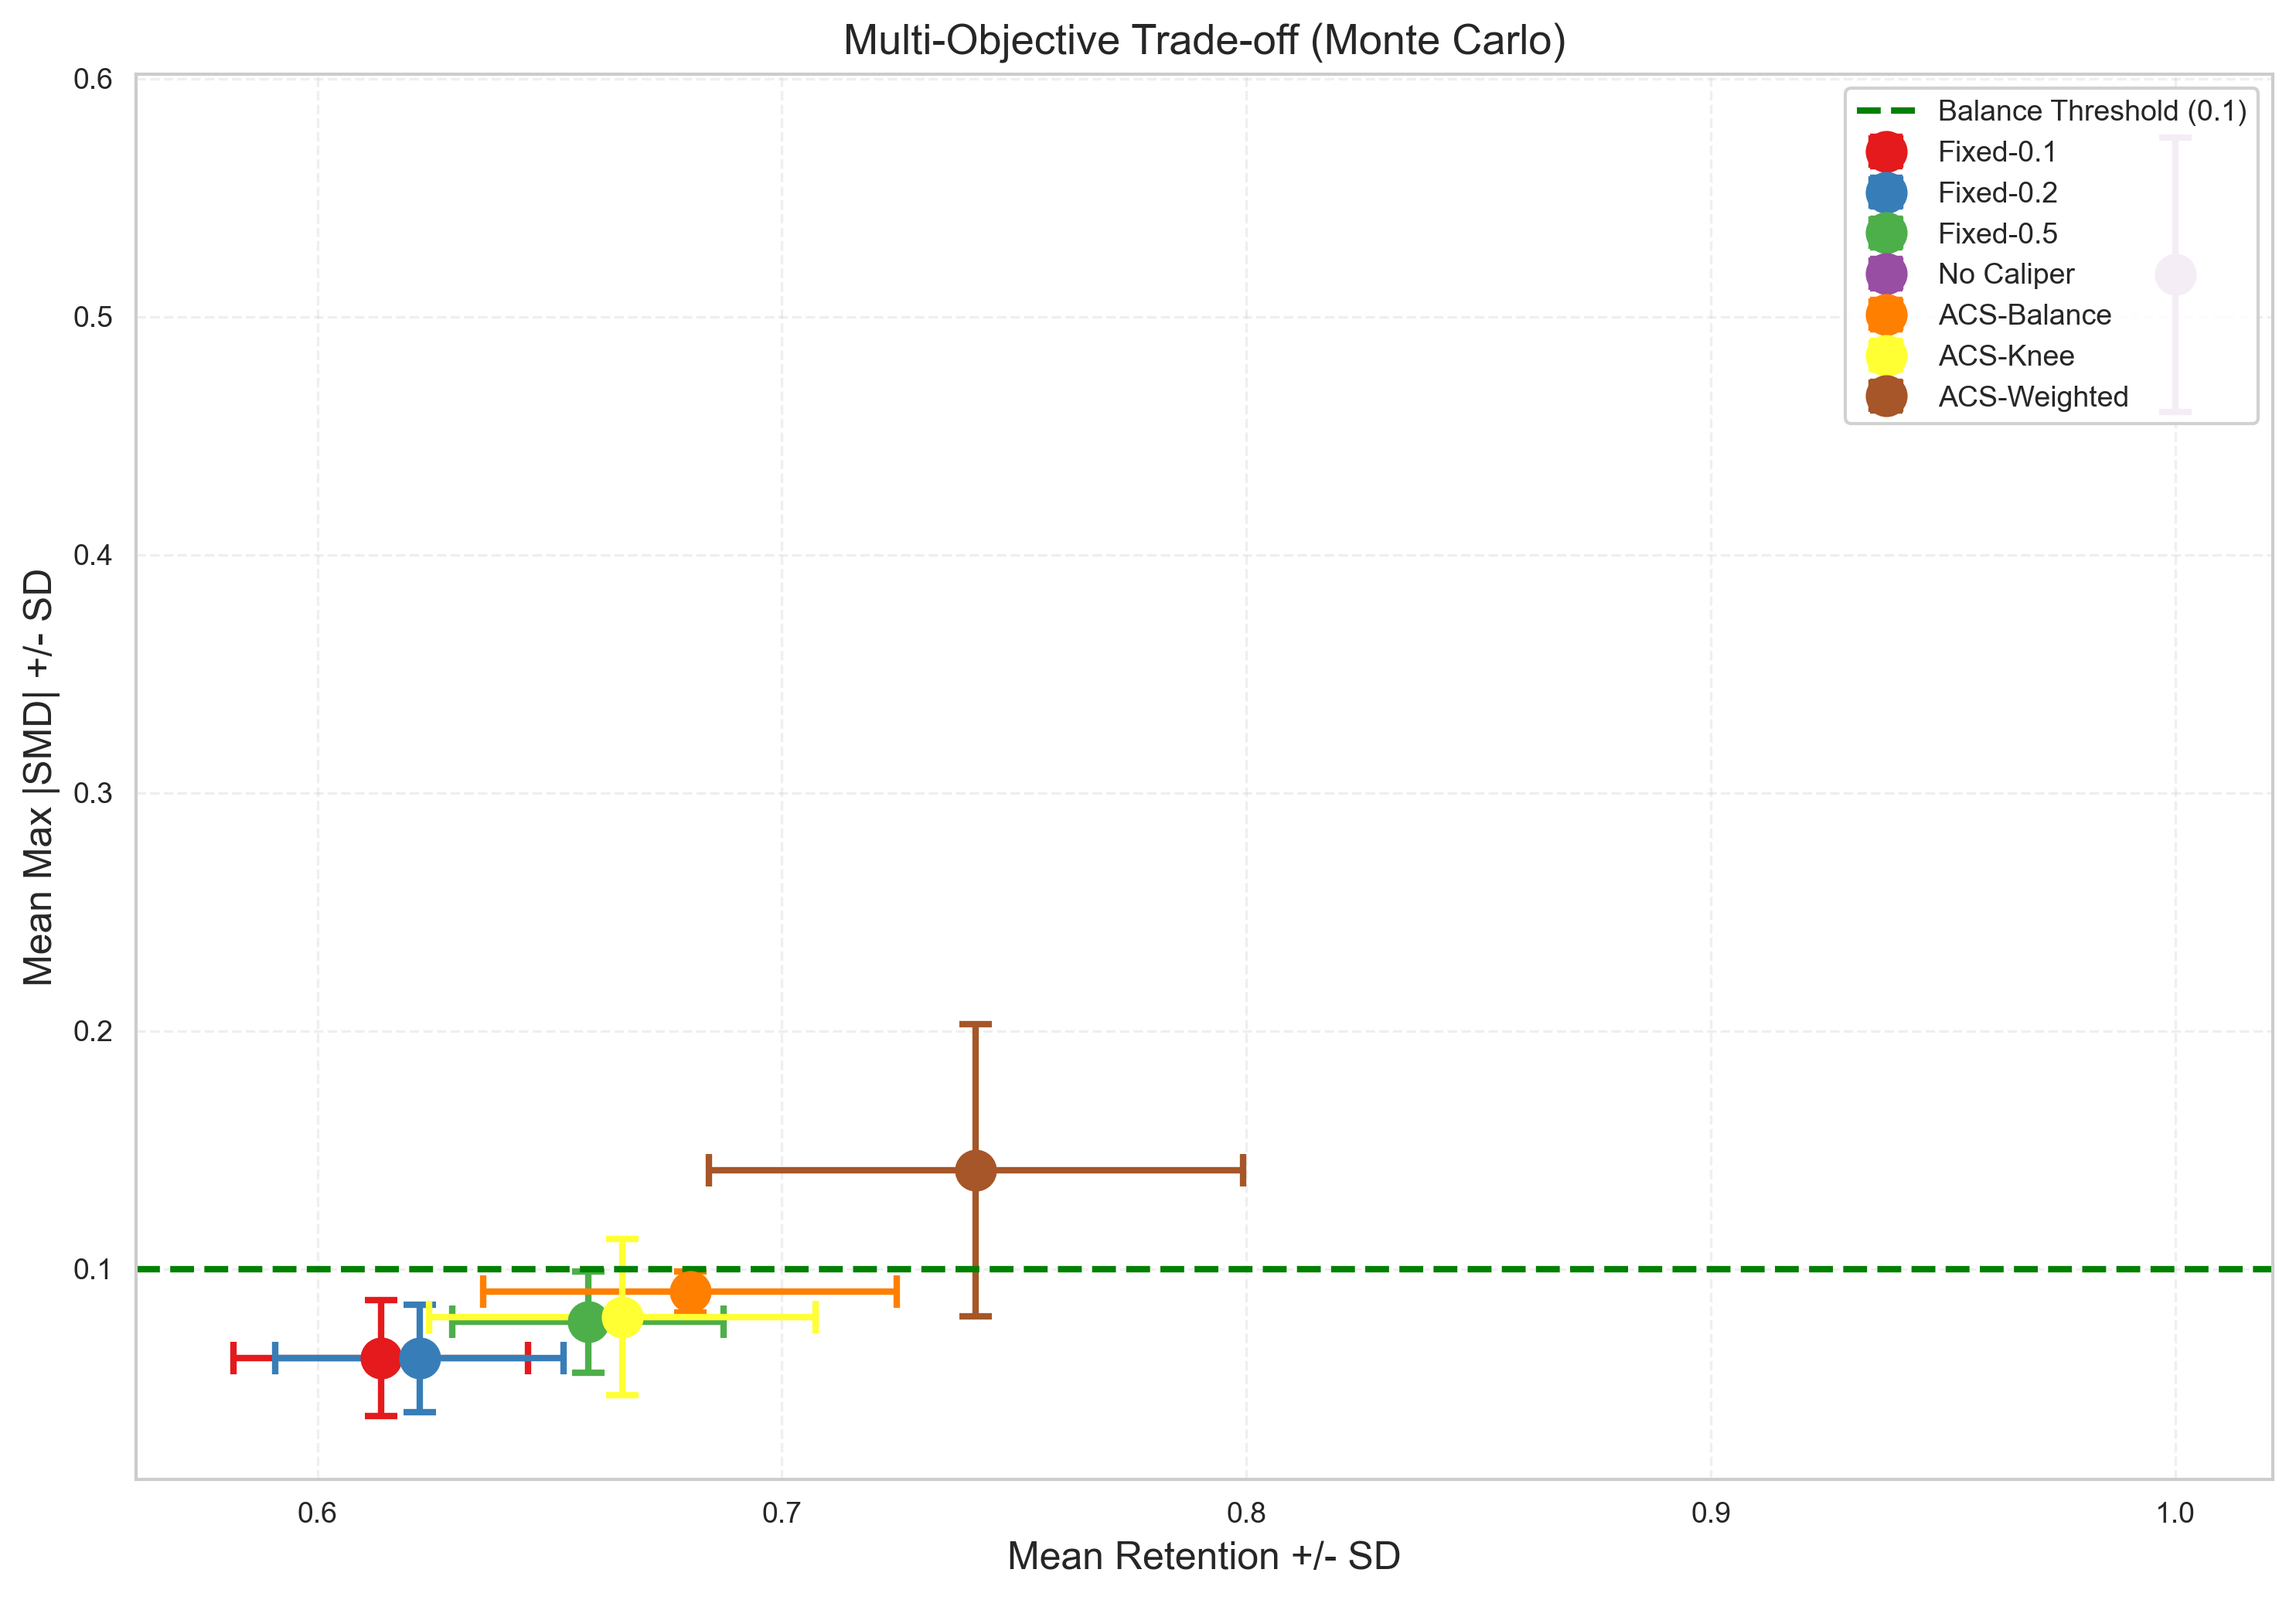
\includegraphics[width=0.75\textwidth]{outputs/figures/fig7_mc_tradeoff.png}
    \caption{Multi-objective trade-off from Monte Carlo simulation. Points show mean balance vs.\ mean retention; error bars indicate $\pm 1$ SD. Dashed line: balance threshold.}
    \label{fig:mc_tradeoff}
\end{figure}

The figure reveals clear method clustering: (1) restrictive fixed calipers (0.1, 0.2) achieve excellent balance with moderate retention; (2) ACS-Knee and ACS-Balance occupy the middle ground; (3) ACS-Weighted and Fixed-0.5 sacrifice balance for retention; (4) No Caliper represents the extreme of maximum retention with unacceptable imbalance.

%% -----------------------------------------------------------------------------
\subsection{Summary of Key Findings}

\begin{enumerate}
    \item \textbf{Pareto frontier characterization}: The balance-retention trade-off is well-characterized by the Pareto frontier, with 11 non-dominated caliper values identified.
    
    \item \textbf{ACS-Knee superiority}: Among adaptive methods, ACS-Knee achieved the best bias-variance trade-off (MSE $= 0.039$, coverage $= 74\%$) while maintaining balance below threshold.
    
    \item \textbf{Fixed caliper competitiveness}: Conservative fixed calipers (0.1--0.2 SD) achieved lowest bias and highest coverage, though at cost of 38--39\% sample loss.
    
    \item \textbf{ACS-Weighted limitations}: Equal weighting of balance and retention ($\lambda = 0.5$) produced inadequate balance, suggesting $\lambda > 0.5$ may be preferable in practice.
    
    \item \textbf{No Caliper failure}: Matching without caliper restriction resulted in severe bias and zero coverage, confirming the necessity of caliper constraints.
\end{enumerate}

%% =============================================================================
%% END OF RESULTS SECTION
%% =============================================================================
